How would you define what a prison is? I would argue most people after some thought would produce a response roughly equivalent to the following: \\

\begin{minipage}{\dimexpr\textwidth-1cm}
	\itshape
	A prison is a secure facility where individuals convicted of crimes are confined as punishment, separated from society to ensure public safety.
\end{minipage} \\

\noindent
However, I offer that the American prison system and arguably prisons in general are an invisible hand of the government that enacts punishment on those at any time it deems as wrongdoers in society. Prisons, both public and privately owned, are not independent entities. While they may have operational autonomy is some cases, its inmates all were sentenced as a result of the courts and consequently the law. Hence, the prison is understood only in the context of the law. As rhetorically asked by Ruth Wilson Gilmore, "But what about crime? Doesn’t prison exist because there are criminals" \cite*[12]{gilmoreGoldenGulagPrisons2007}? Often the idea of a criminal or wrongdoer of society is treated as an objectivity. However, the law is rather a continually changing system that bends and changes according to "who, in a social order, needs to be controlled" \mancite\cite[12]{gilmoreGoldenGulagPrisons2007}. 

\subsubsection*{Invisibility and the Law}
An important part of the characterization I offer of prisons is their \textit{invisibility}. Prisons are invisible in both a physical and mental sense. The locations of prisons are often in rural parts of America because of the limited political opposition, availability of large landholdings, and the access to swaths of former agricultural lands to be developed. Consider the following case. During the 1980s, there was a proposal to construct a prison in East Los Angeles, a highly urban and developed area. There was immediate push back as it would be placed in the middle of a predominantly Mexicano and Chicano community that strongly opposed its construction. Additionally, construction faced the challenge of properly acquiring all the needed land for the prison \cite[103]{gilmoreGoldenGulagPrisons2007}. Contrast this to if a rural environment was chosen. Gilmore notes that the political opposition found in smaller towns when given similar proposals was much lest costly. Additionally, rural regions often had larger landholdings meaning acquiring the acres for development was a more streamlined process. Combined with the fact that around 80\% of Americans live in urban regions, often most people are physically distanced from prisons or potential new prison sites \nocite{UrbanRuralPopulations} ("Urban and Rural\ldots").

Similar to Gilmore's argument about the physical detachment people have from prisons, Davis focuses on the mental detachment many have and the dramatized and distorted perceptions of prisons that form as a result. Davis notes that one often believes they could never be a prisoner themselves. As a consequence, the prison becomes “an abstract site into which undesirables are deposited” \cite*[16]{davisArePrisonsObsolete2003}. Moreover, Davis emphasizes that many people's understanding of prisons is shaped by media portrayals rather than personal experiences or interactions. Davis points out that dramatic interpretations in films like "\textit{I Want to Live}, \textit{Papillon}, \textit{Cool Hand Luke}, and \textit{Escape from Alcatraz}" \cite*[18]{davisArePrisonsObsolete2003} perpetuate a more glamorized and romanticized prison experience, ignoring the harsh realities and injustices that occur day to day inside them. Gilmore's argument has an important connection to Davis' in which the physical distancing of prisons from urban areas helps enable and exacerbate people's mental detachment from prisons. As more prisons are constructed in physically distant locations, fewer people become aware of their presence and rely more on external portrayals and information to inform their understanding of prisons. This invisibility of prisons provides those in power a system that, outside the public eye and conscious, allows the enactment of punishment and exploitation of those imprisoned.

I would like to restate a rhetorical question Gilmore asks: "Doesn't prison exist because there are criminals?" \cite*[12]{gilmoreGoldenGulagPrisons2007}. While my offered definition of prisons may align with the common sense idea that a prison is for wrongdoers and criminals, I believe that the key word is \textit{deemed}. It is at the discretion of the governmental and capitalistic systems who is a wrongdoer and who is not. The classification of criminal or not criminal does not stem from an objective checklist or criteria, but rather a complex system of law and order that often bends to the will of those in power. Returning to Angela Davis, their case studies in \textit{Are Prisons Obselete} serve to highlight how the prison is not an isolated system of oppression but instead plays a larger part in the continuation of anti-blackness from the era of slavery. The prison is one with the law, and the law has always been a vehicle for anti-blackness. An example that Davis points out is the Black Codes. As said by Davis, "The new Black Codes proscribed a range of actions-such as vagrancy, absence from work, breach of job contracts, the possession of firearms, and insulting gestures or acts-that were criminalized only when the person charged was black" \cite*[28]{davisArePrisonsObsolete2003}. It was not uncommon to have curfew laws that specifically targeted African American. In 1714, the New Hampshire general assembly passed an act that stated that "No Indian, Negro, or Molatto is to be from Home after 9 o'clock" \cite{marksammonsBlackPortsmouth2004}. Curfews and laws like the Black Codes came from a place of racial prejudice and power. Motivated by fear, these laws were enacted to suppress emancipated African Americans and do not represent an objective evaluation of any form of criminality, moral corruptness, or any other measure of wrong doing. This example sheds light on the fact that those in prison are sentenced under the law, and the law itself is derived by those in power in ways that are prejudiced.

While the Black Codes were mostly abolished by the Civil Rights Act of 1866, racial inequality and system injustice have persisted. Michelle Alexander expands on this further in her book \textit{The New Jim Crow}. Alexander specifically discusses the "War on Drugs", a campaign with roots in the 1970s that grew in scope under the Reagan Administration and has persisted to this day. The idea of criminality being an objective measure was a core component of what Alexander says Reagan's "'color-blind' rhetoric on crime, welfare, taxes, and states' rights" \cite[47]{alexanderNewJimCrow2012}. In reality, those imprisoned as a result of the resultant laws have been disproportionately African American men. Concerning changes in law, the supreme court played a large role in allowing for easier search and seizure for suspicion of drugs, allowing police to more easily charge people under loose drug possession laws. Alexander notes that in the court decision \textit{Florida v. Bostick}, police officers were allowed to, without suspicion, attempt to gain voluntary consent for a search that could be used against a person in court \cite[63]{alexanderNewJimCrow2012}. Additionally, the Anti-Drug Abuse Act put in place felony charges and minimum sentencing guidelines for offenses such as basic cocaine possession. Alexander goes through numerous case studies where these two aspects and more of the War on Drugs led to the destruction of many African American lives, even if a conviction isn't secured. Just like how Davis draws a connection between the law and criminality in the context of the Black Codes, Alexander establishes the same rhetorical argument through the War on Drugs. Therefore in both Alexander's and Davis' analysis, it can be seen the law serves those in power, and since prisons house those that break the law, the law can be used as a tool by the government and powerful.

\subsubsection*{Motivation for Change}
Based on the prior analysis, I argue that the purpose of prisons is not public safety, but rather a method of those in power to target, punish, and silence whomever it wants. Therefore, if the prison does not serve as method of public safety, is it a necessary component for society to function? Should its long standing history still justify its existence? As Davis asks quite nicely, does a "system that \ldots prevailed during the eighteenth and nineteenth centuries \ldots lay absolute claim on the twenty-first century" \cite[43]{davisArePrisonsObsolete2003}?

\begin{wrapfigure}{r}{0.4\textwidth}
	\centering
	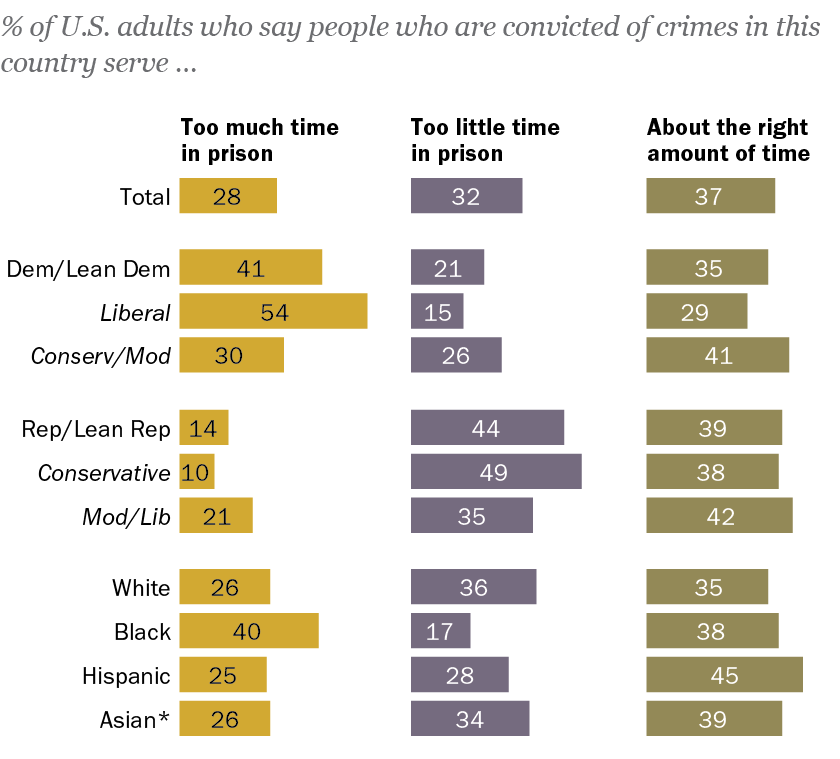
\includegraphics[width=0.4\textwidth]{figures/pewpoll.png}
	\caption{Survey of Americans Opinions on Prison Time}
	\label{fig:pewpoll}
\end{wrapfigure}
As seen in Figure \ref{fig:pewpoll}, a majority of adult Americans (69\%) believe that prisoners are either serving the right amount of time or \textit{too little} time in prison \nocite{AmericansDifferParty}("American Differ by Party\ldots").
Additionally, in 2020 close to 0.7\% of the US population was imprisoned \cite{peterwagnerWhatPercentIncarcerated}. For me, I see these statistics and return back to the common sense definition of a prison from the beginning \textit{A prison is a secure facility where individuals convicted of crimes are confined as punishment, separated from society to ensure public safety}. I consider the question of public safety and ask does the majority opinion that sentencing times are adequate or not enough or the fact that almost 1\% of Americans are in prison reflect the ideals of public safety? I would argue that in the context of the arguments of Davis, Gilmore, and other abolitionists that the answer to this question is no. 

It is important to discuss and engage with these abolitionist perspectives in the present year, especially considering younger generations. Young people are the next in line to inherent the current social order, and consequently they are the ones poised to enact change through mobilization and active advocacy of transformative justice. The embracing of abolitionist ideas can help facilitate the highlighting and resolution of inherent injustices in the current prison system, promotion of empathy and rehabilitation, and undoing of centuries of anti-blackness that plagues prisons to this day.
